% !TEX encoding = UTF-8 Unicode

\documentclass[a4paper]{article} 

% Om du använder pdfLaTeX, inkludera följande två paket, för att få svenska bokstäver och rätt teckenkodning:
% \usepackage[T1]{fontenc}     % För svenska bokstäver
% \usepackage[utf8]{inputenc}  % Teckenkodning UTF8

% Om du använder XeLaTeX så behöver du inte inkludera ovanstående paket.

% Allt nedanför gäller oavsett om du använder pdfLaTeX eller XeLaTeX

\usepackage[swedish]{babel}  % För svensk avstavning och svenska
                             % rubriker (t ex "Innehållsförteckning")
\usepackage{fancyvrb}        % För programlistor med tabulatorer
\fvset{tabsize=4}            % Tabulatorpositioner
\fvset{fontsize=\small}      % Lagom storlek för programlistor
\usepackage{graphicx}



\title{Newton-Raphsons metod}
\author{Per Holm}
\date{21 maj 2001}           % OBS! Vet inte när Per skrev dokumentet, jag hittade på ett datum.

\begin{document}             % Början på dokumentet

\maketitle                   % Skriver ut rubriken som vi definierade ovan med \title, \author, \date

\section{Numeriska metoder}

En \emph{numerisk metod} är en metod med vars hjälp man kan finna en
approximativ lösning till ett matematiskt problem. Lösningen ges i
numerisk form dvs i form av ett antal talvärden. Till exempel kan man
med en numerisk metod räkna ut att roten till ekvationen $x^2 = 3$ är
$1.73205\ldots$, men inte få fram den analytiska lösningen $\sqrt 3$.

I många problem är man hänvisad till numeriska metoder. Det kan
bero på att problemet inte har någon analytisk lösning eller att det
skulle vara alltför arbetsamt att få fram denna.

I denna rapport studeras en numerisk metod för att lösa ekvationer
med en obekant, nämligen Newton-Raphsons metod.\footnote{Metoden kallas ibland Newtons metod.}



\section{Newton-Raphsons metod}


\subsection{Teori}

Vi söker en rot $\alpha$ till ekvationen $f(x) = 0$. Vi antar att vi vet att
roten ligger i närheten av talet $x_0$ och ska försöka förbättra denna
approximativa lösning.  Vi kan bilda nya approximationer $x_1, x_2, x_3,
   \ldots$ med följande formel:

\begin{equation}
   x_{k+1} = x_k - \frac{f(x_k)}{f'(x_k)}
   \label{nrekv}
\end{equation}

\noindent Metoden åskådliggörs geometriskt i figur~\ref{nrbild}. Tangenten i punkten
$(x_0,f(x_0))$ skär x-axeln för $x = x_1$, tangenten i punkten $(x_1,f(x_1))$
skär x-axeln för $x = x_2$, osv. Av figuren förstår vi att $x_k \rightarrow
   \alpha$ då $k \rightarrow \infty$.


Newton-Raphsons metod kan härledas genom att man serieutvecklar
funktionen $f(x_0-\epsilon)$ och trunkerar utvecklingen efter den linjära
termen. Ur serieutvecklingen kan man också få ett uttryck på
feltermen.

\begin{figure}
   \begin{center}
      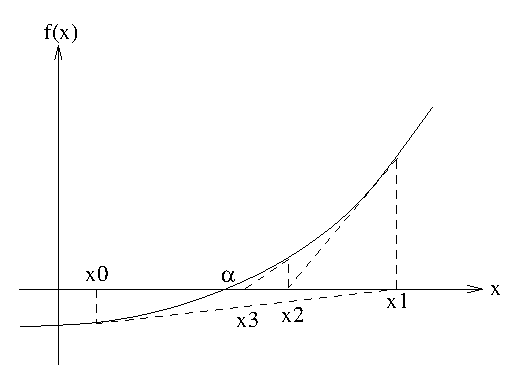
\includegraphics[width=65mm]{nrbild}
   \end{center}
   \caption{Newton-Raphsons metod}
   \label{nrbild}
\end{figure}


\subsection{Exempel}

Ekvationen $e^{-x} = \sin x$ har en rot nära $0.6$. Bestäm denna rot med
Newton-Raphsons metod.

\newpage
Här är $f(x) = e^{-x} - \sin x$, $f'(x) = -e^{-x} - \cos x$. Om vi räknar
med 9 decimaler så får vi:

\medskip
$\begin{array}{llll}
      x           & f(x)         & f'(x)        & f(x)/f'(x)   \\
      0.6         & -0.015830837 & -1.374147251 & 0.011510481  \\
      0.588479519 & 0.000073820  & -1.386956425 & -0.000053224 \\
      0.588532743 & 0.000000001  & -1.386897331 & -0.000000001 \\
      0.588532744                                              \\
   \end{array}$

\medskip
\noindent dvs $\alpha = 0.588532744$.



\subsection{Konvergens}
\label{sec:konv}
Newton-Raphsons metod konvergerar i allmänhet \emph{kvadratiskt} mot den
sökta roten, vilket innebär att antalet korrekta siffror i svaret
fördubblas i varje iteration. Men det finns fall då konvergensen
blir sämre eller då metoden inte alls konvergerar, nämligen då man
råkar ut för en derivata som är nära noll. Två sådana fall illustreras
i figur~\ref{konvbild}.

\begin{figure}[b]
   \begin{center}
      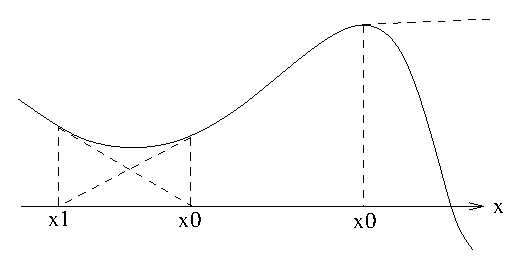
\includegraphics[width=70mm]{konvbild}
   \end{center}
   \caption{Konvergensproblem}
   \label{konvbild}
\end{figure}



\section{Newton-Raphsons metod i Java}

Det är inte helt enkelt att implementera Newton-Raphsons metod i ett
program, åtminstone inte om man kräver att metoden ska fungera i
alla upptänkliga fall.  I metoden \texttt{solve} som visas nedan finns bara
den grundläggande algoritmen med: vi har inte tagit hänsyn till
undantagsfall som finns eller fel som kan inträffa, till exempel
att derivatan \texttt{fprim(x0)} blir nära noll (se avsnitt~\ref{sec:konv}).

\VerbatimInput{NewtonRaphson.java}

\end{document}               % Slut på dokumentet
